\subsection{Modifying the compiler backend}
\label{backend}

First, we had to make a new version of the code generator. The compiler now outputs a JSON file, containing the elements described below.

\begin{itemize}
\item The list of the classes that the program contains
\item For each class, the list of its methods
\item For each method
	\begin{itemize}
	\item the variables declared in it
	\item the arguments list, along with their type
	\item the code
	\end{itemize}
\end{itemize}

The code is a simplified bytecode-like language (in its textual representation), whose full specification can be found in the file \textsc{ASM\_definition.md} (Github link at the end of the document). The opcodes are similar to the ones found in Java's bytecode, with several notable differences.

\begin{itemize}
\item variables, methods and classes are referred to by their name, and not a numeric identifier
\item an instruction \textsc{stat} is used to map instructions to source code lines
\item locales are resolved at runtime
\end{itemize}

This bytecode-like language seemed to be the best solution. First, we could have transpiled directly to JavaScript and use some JS magic to allow the step-by-step execution. While it could seem like a feasible solution at first, due to the highly dynamic nature of JS, it is in practice not possible to break a function call to allow for instance \textit{step into} and \textit{step out} operations. This means that we need to create a machine able to execute the code with a clean debugging interface. We could also have interpreted the tool code directly, but since we already have a compiler for tool, it allows us to implement a very simple stack machine --- which is way easier than a complete tool interpreter. This justifies our choice regarding this low-level code representation.

%If you are using theoretical concepts, explain them first in this subsection.
%Even if they come from the course (eg. lattices), try to explain the essential
%points \emph{in your own words}. Cite any reference work you used like this
%\cite{TigerBook}. This should convince us that you know the theory behind what
%you coded.



\subsection{Porting the compiler in the browser}

To make the compiler run in the browser, we used \textsc{ScalaJS}, an EPFL-made library that transpiles Scala to JavaScript.
It needs however some bindings to properly interact with our JavaScript code. We wanted to make as few modifications as possible to the compiler's CLI interface. To this end, we used BrowserFS, a library that creates a NodeJS style file system interface, and created a few simple nodejs-scala bindings so that this interface could be used instead of java's file system. The compiler code can then be kept intact and will work as expected when run in a browser. It worked well for input files but got a little dirty as far as output was concerned. We therefore opted for a more invasive technique. A JS function in charge of receiving the compilation output is called directly in the code generation stage of the compiler which makes this specific version of the compiler unusable outside the web IDE.

\paragraph{}
This work of porting the compiler to the browser makes a huge difference in terms of usability of our debugger. It becomes almost a minimalist IDE for tool. We can compile as the code is typed and report errors in the editor, thanks to the positioned error reporting previously implemented in the compiler.

\subsection{Implementation of the virtual machine}

At this stage, we had a compiler able to run in the browser and output a custom representation of any Tool program, but nothing to interpret it.
We have implemented a JavaScript virtual machine able to execute instructions that we have defined for our custom bytecode-like language.

\subsubsection{Architecture}

The execution is handled by the Engine class. It contains a StateMachine and methods to handle the debugging control flow (breakpoints, run, step into, etc.).
The state machine contains information about the current state of the program (stack, program counter, current scope...) as well as methods to change it.\\

\begin{figure}[h]
  \centering
    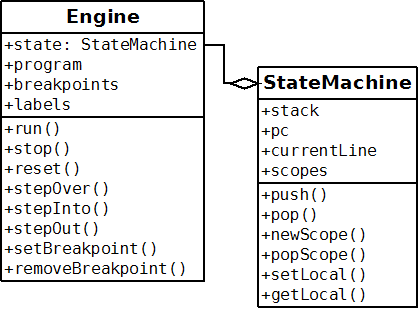
\includegraphics[scale=0.6]{diag.png}
     \caption{(Non-exhaustive) class structure}
\end{figure}

\subsection{Developing the web interface}

After that, we had to implement the web interface of the debugger. It is divided into four main parts.

\begin{itemize}
\item The code editor, where you can type code and set breakpoints
\item The toolbar, which allows you to load a Tool source file, compile it, and control the debugging process (run / stop / step over / step into / step out)
\item The console, where you can see messages from the debugger, compilation errors, and the program output
\item The right panel, that allows you to see the values of the variables in the current scope, the call stack and the breakpoints you have set. Clicking on an element of the call stack will bring you at the location the call was made. Breakpoints can be disabled by clicking on the green dot icon, and removed with a right click.
\end{itemize}

The interface was made in HTML and JavaScript, with the use of \href{http://dojotoolkit.org/reference-guide/1.10/dijit/}{Dijit}, a popular library to create web user interfaces.

A special tab entitled \textit{ASM} allows you to see what \textit{bytecode-like} code was generated. It is not relevant when debugging a tool program, but can be useful to see what's happening behind the scenes. It will have at least allowed us to debug the debugger.

\subsubsection{Control flow}

Once the tool code has been typed, it can be debugged using the control buttons at the top of the interface.

\paragraph{}
The run action runs the program. As everything (debugger and virtual machine) is single threaded, there is no way to stop a program that loops forever if no breakpoints have previously been set.\\
The stop action resets the program. One must click on the stop button to reset the program once it has run before running it again.\\
The left arrow --- \textit{step over} action --- steps over the current line. \\
The down arrow --- \textit{step into} action --- steps into the current function call. If the current instruction is not a function call, it goes to the next instruction.\\
The up arrow --- \textit{step out} action --- steps out of the current function call, returning to the line where the function has been invoked.
If there are multiple function calls in one instruction, one can use a combination of step into/step out to visit each call.

\paragraph{Breakpoints}
The last control flow feature is breakpoints. To set a breakpoint, one can click on the left gutter, next to the line number corresponding to the line you want to break on. Note that not every line is breakable. You can only break on actual statements. Once a breakpoint has been set, it can be removed by clicking again on the same spot. A breakpoint can also be disabled by clicking the green icon in the breakpoints view on the right, making it ineffective but still set for later use. The debugger will always stop at an active breakpoint when its line is reached.
\\
Breakpoint rules takes precedence over action rules, i.e. if a \textit{step out} action is requested but there's a breakpoint before the end of the function, the execution will pause at the line where the breakpoint is set.
